\documentclass[a4paper]{article}
\usepackage[12pt]{extsizes}
\usepackage[utf8]{inputenc}
\usepackage[T2A]{fontenc}
\usepackage{amssymb,amsmath,mathtext}
\usepackage{indentfirst,amsfonts}
\usepackage[english, russian]{babel}
\usepackage{setspace,amsmath}
\usepackage{graphicx}
\usepackage[left=30mm, top=20mm, right=10mm, bottom=20mm, nohead, footskip=10mm]{geometry} % настройки полей документа

\graphicspath{{graphs/}}

\begin{document}
	\begin{titlepage} % начало документа
		
		% НАЧАЛО ТИТУЛЬНОГО ЛИСТА
		\begin{center}
			\footnotesize{ФЕДЕРАЛЬНОЕ ГОСУДАРСТВЕННОЕ БЮДЖЕТНОЕ ОБРАЗОВАТЕЛЬНОЕ }\\ 
			\footnotesize{УЧРЕЖДЕНИЕ ВЫСШЕГО ОБРАЗОВАНИЯ}\\
			\small{«МОСКОВСКИЙ ГОСУДАРСТВЕННЫЙ УНИВЕРСИТЕТ}\\
			\small{имени М.В.ЛОМОНОСОВА»}\\
			\hfill \break
			\normalsize{ФИЗИЧЕСКИЙ ФАКУЛЬТЕТ}\\
			\hfill \break
			\normalsize{КАФЕДРА МАТЕМАТИЧЕСКОГО МОДЕЛИРОВАНИЯ И ИНФОРМАТИКИ}\\
			\hfill \break
			\hfill \break
			\hfill \break
			\hfill \break
			\hfill \break
			\hfill \break
			\large{\textbf{Нейросетевой синтез текстур с трендами}}\\
		\end{center}
		
		\hfill \break
		
		\begin{flushright}
			Выполнил студент \\
			\hfill \break
			435 группы:\\
			\hfill \break
			Будакян Я. С.\\
			\hfill \break
			\hfill \break
			\hfill \break
			Научный руководитель: \\
			\hfill \break
			к.т.н., доц. Грачев Е. А.\\
			\hfill \break
		\end{flushright}
		
		\hfill \break
		\hfill \break
		\hfill \break
		\hfill \break
		\hfill \break
		\hfill \break
		
		\begin{center}
			Москва \\
			\hfill \break
			2017 
		\end{center}
		
		\thispagestyle{empty} % выключаем отображение номера для этой страницы
		
		% КОНЕЦ ТИТУЛЬНОГО ЛИСТА
		
	\end{titlepage}  % КОНЕЦ ДОКУМЕНТА !
	%учитываем титульный лист в нумерации
	\setcounter{page}{2}
	\section{Введение}
		Задача состоит в синтезе изображений среды, которые будут содержать в себе тренд, т.е. изменение некоторой статистической характеристики. Такими трендами могут быть, например, изменение интенсивности появления частиц среды вдоль изображения, или изменение пористости среды. \\
		\begin{figure}[h]
			\centering{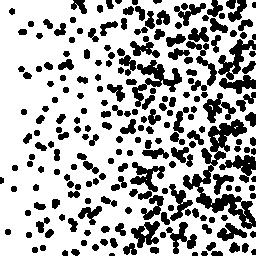
\includegraphics[width=0.35\linewidth]{trend-sample}}
			\caption{Пример текстуры с трендом интенсивности частиц}
		\end{figure}
	\section{Математическая постановка}
		С математической точки зрения, задача сводится к синтезу случайного изображения $X'$ (и построению соотвествующей процедуры синтеза), принадлежащему распределению, близкому к желаемому:
		$$ P_{X'} \approx P_X,$$
		где $P_X$ - распределение изображений с трендами, удовлетворяющих следующим ограничениям (для упрощения задачи):
		\begin{itemize}
			\item Это монохромные изображения 256 x 256 пикселей
			\item Изменяющимся свойством является интенсивность появления частиц $\lambda$
			\item Тренд является линейным и направлен вдоль оси x: 
			$ \lambda = \lambda_0 + kx $
		\end{itemize}
		Распределение $P_X$ задается обучающей выборкой.
	\section{Существующие подходы к решению задачи}
		Есть несколько подходов к решению задач подобного рода:
		\begin{itemize}
			\item 'Классический' статистический подход
			\item Базовый нейросетевой подход
			\item Генеративные состязательные сети (GAN)
		\end{itemize}
		\subsection{'Классический' статистический подход}
			\begin{itemize}
				\item Вводится параметризированное семейство распределений вероятности $P_{\theta}(x)$
				\item Параметры $\theta$ находятся из обучающей выборки:
				$$ \mathcal{L}_{\theta}(D) = \prod_{x \in D} P_{\theta}(x) $$
				$$ \theta^{*} = \underset{\theta}{\arg\max} \mathcal{L}_{\theta}(D)$$
				\item Сгенерировать семпл из $ P_{\theta^{*}}$
			\end{itemize}
			Этот подход приводит к проблемам:
			\begin{itemize}
				\item Пространство параметров $\theta$ может быть огромной размерности
				\item Или же известной параметрической модели распределения может вообще не существовать
			\end{itemize}
			Простой пример - генерирование человеческих лиц, похожих на реальные: параметрической модели для такой задачи не существует.
		\subsection{Базовый нейросетевой подход}
			\begin{itemize}
				\item Вводится параметризированное семейство распределений вероятности $P_{\theta}(x)$
				\begin{itemize}
					\item Вводятся скрытые переменные $V$ и функция(нейросеть) для получения $x$ из $V$ (фактически, классификация, развернутая в другую сторону)
				\end{itemize}
				\item Определяются параметры распределения (т.е. обучение нейросети)
				\item Генерируются семплы из $ P_{\theta^{*}}$
			\end{itemize}
			Этот подход возможен, однако на практике трудноосуществим.
		\subsection{GAN - генеративные состязательные сети}
				Вернемся к изначальной задаче: найти процеруду генерирования $X'$ так, чтобы $ P_{X'} \approx P_X$.
				Переформулируем:
				$$ \rho(P_{X'}, P_X) \longrightarrow \underset{P_{X'}}{\min} $$
				Введем некоторые скрытые переменные с фиксированным распределением, например
				$$ V \sim U^n [-1, 1], $$
				и параметризированную процедуру генерации:
				$$ X' = g_{\theta}(V) $$
				Переформулируем:
				$$ \rho(P_{X'}, P_X) \longrightarrow \underset{P_{X'}}{\min} $$
				$$ \rho(g_{\theta}(V), P_X) \longrightarrow \underset{g_{\theta}(V)}{\min} $$
				$$ \rho(g_{\theta}(V), P_X) \longrightarrow \underset{\theta}{\min} $$
				Остается вопрос: что использовать в качестве метрики похожести двух распределений $\rho$, где одно из распределений задано обучающей выборкой.
				В качестве метрики статистической похожести можно использовать loss-функцию обученного классификатора:
				$$ \rho(P_{X'}, P_X) \longrightarrow \min \Leftrightarrow \mathcal{L} \longrightarrow \max, $$
				где $\mathcal{L}$ - функция потерь обученного классификатора.
				Соответственно, можно ввести две нейросети:
					\begin{itemize}
						\item $d_{\zeta}(x)$ - классификатор для измерения расстояния, \textbf{дискриминатор}
						\item $g_{\theta}(x)$ - сеть, трансформирующая $V$ в $X'$, \textbf{генератор}
					\end{itemize}
					Введем loss-функцию дискриминатора(например, кросс-энтропия):
					$$ L(X, X') = \frac{1}{2} \mathbb{E}_{x \sim X} l(d_{\zeta}(x), 1) + \frac{1}{2} \mathbb{E}_{x' \sim X'} l(d_{\zeta}(x'), 0) = $$
					$$ = -\frac{1}{2} (\mathbb{E}_{x \sim X} \log d_{\zeta}(x) + \mathbb{E}_{x' \sim X'} \log (1 - d_{\zeta}(x'))) = $$
					$$ =  -\frac{1}{2} (\mathbb{E}_{x \sim X} \log d_{\zeta}(x) + \mathbb{E}_{v \sim V} \log (1 - d_{\zeta}(g_{\theta}(v)))) = $$
					$$ = L(\zeta, \theta) $$
					Loss-функция обученного классификатора:
					$$ L^*(\theta) = \underset{\zeta}{\min} L(\zeta, \theta) $$
					Соответственно,
					$$ \underset{\zeta}{\min} L(\zeta, \theta) \longrightarrow \underset{\theta}{\max} $$
					$$ \theta^* = \underset{\theta}{\arg\max} \left[ \underset{\zeta}{\min} L(\zeta, \theta) \right] $$
					Определим оптимальный дискриминатор:
					$$ d^*_{\theta} = d_{\zeta^*(\theta)} $$
					$$ \zeta^*(\theta) =  \underset{\zeta}{\arg\min} L(\zeta, \theta)$$
	\section{Обучение GAN}
		Итак, задача обучения GAN свелась к нахождению
		$$ \theta^* = \underset{\theta}{\arg\max} \left[ \underset{\zeta}{\min} L(\zeta, \theta) \right] $$
		Решить ее можно, например, методом стохастического градиентного спуска:
		$$ \Delta \theta \sim \nabla L(\zeta^*(\theta), \theta)$$
		Для малых изменений $\Delta \theta$:
		$$ \nabla L(\zeta^*(\theta), \theta) \approx \nabla L(\zeta^*(\theta), \theta + \Delta \theta) $$
		В итоге, процесс обучения принимает следующий вид:
		\begin{itemize}
				\item Обучаем дискриминатор при 'замороженном' генераторе
				\item Обучаем генератор при 'замороженном' дискриминаторе
				\item Повторяем много раз
		\end{itemize}
		\begin{figure}
			\begin{center}
				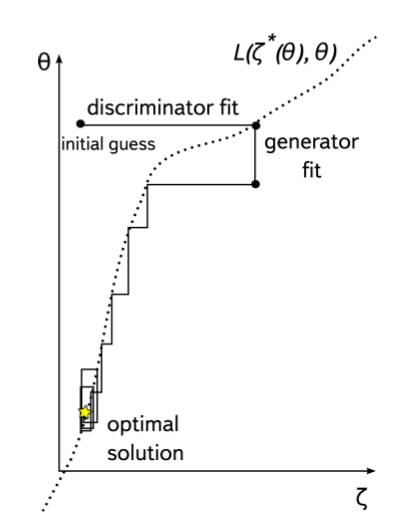
\includegraphics[width=0.4\linewidth]{gan-training}
			\end{center}
			\caption{Схематическое изображение процесса обучения GAN}
		\end{figure}
	\section{pix2pix GAN}
		Для решения задачи было попробовано применить модификацию GAN-сети по названием "pix2pix GAN". Для нее функционал потерь выглядит следующим образом: $$ \mathcal{L}(G, D) = \mathcal{L}_{adv}(G, D) + \eta \mathbb{E}_{s_1, s_2, r \sim p_{data}(s_1, s_2, r)} (\parallel r - G(s_1, s_2) \parallel_1)$$
		$$ \mathcal{L}_{adv}(G, D) = \mathbb{E}_{s_1, s_2, r \sim p_{data}(s_1, s_2, r)}\log D(s_1, s_2, r) + $$ $$ + \mathbb{E}_{s_1, s_2 \sim p_{data}(s_1, s_2)} \log (1 - D(s_1, s_2, G(s_1, s_2)))$$
		где G, D - генератор и дискриминатор, $(s_1, s_2, r)$ - тройка изображений (интенсивность слева, справа и реальное изображение с трендом),  $\mathbb{E}_{s_1, s_2, r \sim p_{data}(s_1, s_2, r)}$ - мат. ожидание логарифмического правдоподобия того, что тройка изображений $(s_1, s_2, r)$ принадлежит вероятностному распределению реальных троек $p_{data}(s_1, s_2, r)$, а $p_{data}(s_1, s_2)$ соответствует распределению реальных изображений $s_1, s_2$.
		\begin{figure}[h]
			\begin{center}
				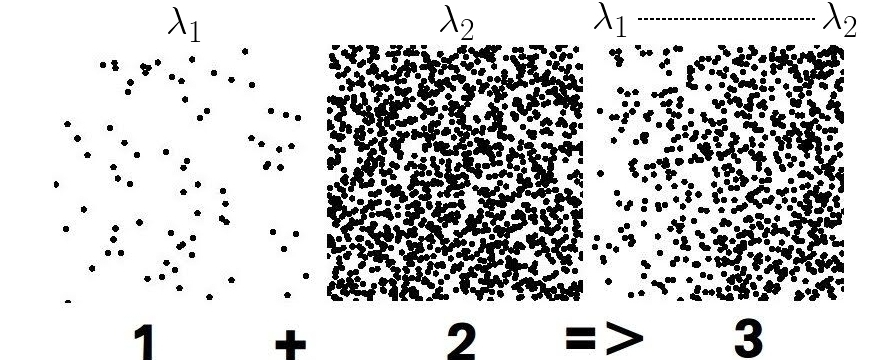
\includegraphics[width=0.75\linewidth]{p2p-gen}
			\end{center}
			\caption{Вход и желаемый выход нейросети}
		\end{figure}
	\section{Критерий качества}
		После обучения генератора, необходимо проверить, что сгенерированные им изображения действительно имеют искомые характеристики. Для этого нужно ввести специальную метрику, которая будет учитывать наличие в изображении тренда интенсивности частиц. Было решено использовать среднюю плотность черных пикселей в некотором окне, и проходить этим окном по изображению (Рис. 4):
		$$\xi_k = \frac{1}{H w}{\sum_{i=k}^{k+w} \sum_{j=0}^{H}\left| \frac{x(i, j) - 255}{255} \right|}, $$$$k = \overline{1, W - w + 1} $$
		\begin{figure}[h!]
			\begin{center}
				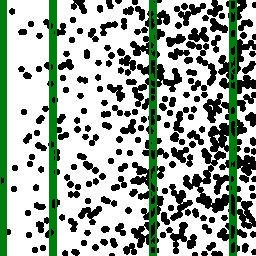
\includegraphics[width=0.35\linewidth]{metrics}
			\end{center}
			\caption{Прохождение окном, W, H - размеры изображения, w - ширина окна}
		\end{figure}
		\\
		Построив график $\xi(k)$ можно увидеть, как меняется плотность пикселей и прослеживается ли тренд. В качестве метрики можно взять среднеквадратичную ошибку:
		$$ \xi = \frac{1}{W-w}\sum_{k=1}^{W-w+1} (\xi_k - \xi_{0k})^2,$$
		где $\xi_{ok}$ - $\xi_k$, усредненное по примерам из обучающей выборки.
	\section{Результаты}
\end{document}